\documentclass[12pt,letterpaper]{article}
\usepackage[utf8]{inputenc}
\usepackage{amsmath}
\usepackage{amsfonts}
\usepackage{amssymb}
\usepackage{amsthm}
\usepackage{graphicx}
\usepackage{tabularx}
\usepackage[left=2cm,right=2cm,top=2cm,bottom=2cm]{geometry}
\usepackage{multicol}
\usepackage{listings}
\lstset{ 
basicstyle = \ttfamily,
showstringspaces=false,
columns=fullflexible,
frame = single,
literate={*}{{\char42}}1
         {-}{{\char45}}1
         {"}{{\fontencoding{T1}\selectfont\textquotedbl}}1
         {'}{{\fontencoding{T1}\selectfont\textquotesingle}}1
}
\usepackage{lastpage}
\usepackage{fancyhdr}
\usepackage{multirow,array}
\usepackage{newtxtext,newtxmath}
\usepackage{lastpage}
\usepackage{enumitem}
\newcolumntype{Y}{>{\centering\arraybackslash}X}
\pagestyle{fancy}
\fancyhf{}
\lhead{\textsc{BHCC Mat-181}}
\chead{\textsc{Answers}}
\rhead{\textsc{HW Exercises 4.1-4.6}}
\rfoot{Page \thepage ~of \pageref{LastPage}}
\setenumerate[1]{label={\bf 4.\theenumi: }}
\setenumerate[2]{label={\bf (\theenumii): }}
\setenumerate[3]{label={\bf \theenumiii: }}

\begin{document}
\newcommand{\N}[2]{\mathcal{N}\big(#1,~#2\big)}
\newcommand{\Geo}[1]{\texttt{Geo}\big(#1\big)}
\newcommand{\B}[2]{\mathcal{B}\big(#1,~#2\big)}
\newcommand{\AND}{\textsc{~and~}}
\newcommand{\OR}{\textsc{~or~}}


\begin{enumerate}
%\setcounter{enumi}{30}
\item \begin{enumerate}
\item mean
\item mean
\item proportion
\item mean
\item proportion
\end{enumerate}

\item \begin{enumerate}
\item proportion
\item mean
\item proportion
\item proportion
\item mean
\end{enumerate}

\item \begin{enumerate}
\item Point estimate of mean is 13.65 credits. Point estimate for median is 14 credits.
\item Point estimate of standard deviation is 1.91 credits. The point estimate for IQR is 2.
\item $13.65+2*1.91 = 17.47$. So, 16 credits is not unusually high but 18 credits is.
\item Nope. There is natural fluctuation between samples.
\item To calculate standard error...
$$SD_{\bar{x}} \approx \frac{s}{\sqrt{n}} = \frac{1.91}{\sqrt{100}} = 0.191 $$
\end{enumerate}

\item \begin{enumerate}
\item 171.1 centimeters. 170.3 centimeters.
\item 9.4 cm. 14 cm.
\item Nope, 180 is only about 1 standard deviation from the same mean. 155 is less than 2 standard deviations from the mean. Neither is more than 2 standard deviations from the mean.
\item Nope. I'd expect the new statistics to be close but not exactly the same.
\item We use the standard error. $$SE=SD_{\bar{x}} = \frac{\sigma}{\sqrt{n}} \approx \frac{s}{\sqrt{n}} = \frac{9.4}{\sqrt{507}} = 0.417 $$
\end{enumerate}

\item \begin{enumerate}
\item A sampling distribution. 
\item Hmm... well, we kind of needed material from chapter 4.2 to answer this question. 
\begin{verbatim}
Central Limit Theorem, informal description
 If a sample consists of at least 30 independent observations 
 and the data are not strongly skewed, then the distribution
 of the sample mean is well approximated by a normal model.
\end{verbatim}
Now, we might actually expect our data to be skewed. (I have no idea about the habits of hens.) Maybe most hens lay few eggs while a few hens lay many eggs. We can build a probability distribution with a strong skew that maintains $\mu\approx 35$ and $\sigma \approx 18.2$.

Let's say that about $\frac{1}{45}$ hens lay a bunch of eggs, while $\frac{44}{45}$ hens each lay a few eggs. Let $X$ represent the number of eggs laid by a random hen. Let $a$ represent the small number of eggs and $b$ represent the big number of eggs.

\begin{center}
\begin{tabular}{|c|c|}\hline
$x_i$ & $P(X=x_i)$ \\ \hline
$a$   &  $44/45$\\
$b$   &  $1/45$ \\\hline
\end{tabular}
\end{center}

$$E(X) = \frac{44a}{45} + \frac{b}{45} = 35$$
$$SD(X) = \sqrt{\frac{44(a-35)^2}{45}+\frac{(b-35)^2}{45}} = 18.2$$

I will use Maxima, a CAS (computer algebra system), to solve this system.
\begin{verbatim}
(%i13) solve([44*a/45+b/45=35, 44*(a-35)^2/45+(b-35)^2/45=18.2^2],
             [a,b]),numer;
(%o13) [a = 32.25624676434235, b = 155.7251423689365]
\end{verbatim}

\begin{center}
\begin{tabular}{|c|c|}\hline
$x_i$ & $P(X=x_i)$ \\ \hline
$32$   &  $44/45$\\
$156$   &  $1/45$ \\\hline
\end{tabular}
\end{center}

So, now let's see what happens if I make a sampling distribution (with $n=45$) from this population.

Here is my R script:
\begin{lstlisting}[language=r]
X = function(){
    if(runif(1) < 44/45){
        return(32)
    }
    else{
        return(156)
    }
}

Y = function(){
    total = 0
    for(i in 1:45){
        total = total + X()
    }
    return(total/45)
}

means = c()
for(i in 1:10000){
    means = c(means, Y())
}

hist(means, freq=FALSE, main="10000 repetitions of sampling 45 hens", 
     xlab="average number of eggs from a sample of 45 hens")
\end{lstlisting}

The above code generates the following histogram.

\begin{center}
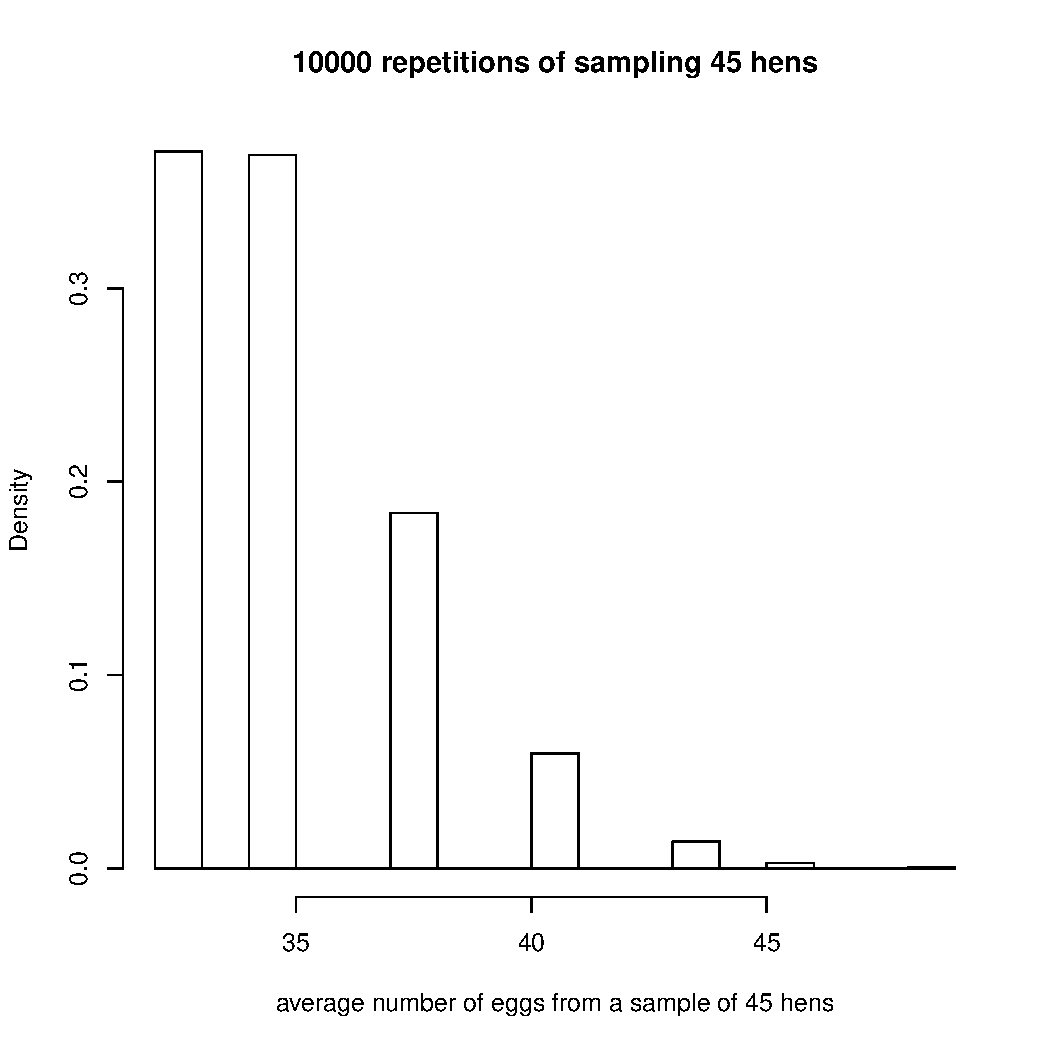
\includegraphics[scale=0.8]{code/hens.pdf}
\end{center}

We see that this (contrived) population will still generate a skewed sampling distribution when $n>30$. But, we probably would have been warned if the data seemed this skewed.

In short, the problem statement left off any description of how skewed the data seemed. Without knowing this, we can't say much about the symmetry of the sampling distribution. If we assume the data seemed nearly symmetric, then we can say the sampling distribution is  symmetric.

\item The question is asking us to calculate the standard error. 
$$SE = SD_{\bar{x}} = \frac{\sigma}{\sqrt{n}} = \frac{18.2}{\sqrt{45}} = 2.71 $$

\item The variability of the new sampling distribution will be larger than the variability of the original sampling distribution. 
$$SE = SD_{\bar{x}} = \frac{\sigma}{\sqrt{n}} = \frac{18.2}{\sqrt{10}} = 5.76 $$
\end{enumerate}

\newpage

\item I felt a bit confused. My interpretation is that 15 people are asked, and a proportion is found; this is repeated 100 times, and a distribution of {\bf proportions} is found. The problem is the author says, ``They repeated this 100 times and built a distribution of sample {\bf means}.'' I guess a proportion is a mean of 0s and 1s... so I guess I shouldn't be confused at all.


\begin{enumerate}
\item A sampling distribution. In this case, we expect the sampling distribution to be related to a binomial distribution. (The binomial distribution is a sum of Bernoulli variables. The proportion sampling distribution is a sum of Bernoulli variables \emph{divided by sample size}.) 

Because they recorded the sample proportion (not the count), our distribution will have outcomes between 0 and 1  (not between 0 and 15). This is the only difference between a proportion sampling distribution and a binomial distribution.

Let me try to spell this out more clearly. Let $W$ represent whether a single student will say yes. Let $X$ represent the number of students who say yes when 15 are asked. Let $Y$ represent the proportion of students who say yes when 15 are asked.

$W\sim Bernoulli(p)$, where $p$ is approximately $14/15 \approx 0.93$. Let's just move forward assuming $p=0.93$, and simulate the expected results. $W\sim Bernoulli(0.93)$.

\begin{center}
\begin{tabular}{|c|c|}\hline
$w_i$ & $P(W=w_i)$ \\ \hline
$0$   &  $0.07$\\
$1$   &  $0.93$ \\\hline
\end{tabular}
\end{center}

$X\sim \B{15}{0.93}$. Remember, a binomial distribution is the sum of many Bernoulli variables. We know how to find the possibilities and their probabilities. 
$$P(X=k) ~~=~~ {15 \choose k}(0.93)^{k}(0.07)^{15-k} $$


\begin{center}
\begin{tabular}{|c|c|}\hline
$x_i$ & $P(X=x_i)$ \\ \hline
$0$   &  $0.00$\\
$1$   &  $0.00$\\
$2$   &  $0.00$\\
$3$   &  $0.00$\\
$4$   &  $0.00$\\
$5$   &  $0.00$\\
$6$   &  $0.00$\\
$7$   &  $0.00$\\
$8$   &  $0.00$\\
$9$   &  $0.00$\\
$10$   &  $0.00$\\
$11$   &  $0.01$\\
$12$   &  $0.07$\\
$13$   &  $0.20$\\
$14$   &  $0.38$\\
$15$   &  $0.34$\\
\hline
\end{tabular}
\end{center}

$Y =  \frac{X}{15} $. In order to convert the number of successes into proportion of success, we divide by the sample size. Notice, only the outcomes are changed, not the probabilities.

\begin{center}
\begin{tabular}{|c|c|}\hline
$y_i$ & $P(Y=y_i)$ \\ \hline
$0$   &  $0.00$\\
$0.07$   &  $0.00$\\
$0.13$   &  $0.00$\\
$0.20$   &  $0.00$\\
$0.27$   &  $0.00$\\
$0.33$   &  $0.00$\\
$0.40$   &  $0.00$\\
$0.47$   &  $0.00$\\
$0.53$   &  $0.00$\\
$0.60$   &  $0.00$\\
$0.67$   &  $0.00$\\
$0.73$   &  $0.01$\\
$0.80$   &  $0.07$\\
$0.87$   &  $0.20$\\
$0.93$   &  $0.38$\\
$1.00$   &  $0.34$\\
\hline
\end{tabular}
\end{center}

This last probability distribution is what we expect the sampling distribution to approach as the repetitions  increase (each repetition is a sample of size 15).

\item 
Right away, we can use the rule-of-thumb for binomial distributions. We need $np>10$ and $n(1-p)>10$ to apply the normal approximation. In this case, $15(1-0.93) = 1$, which is much less than 10. Also, because $p$ is far from 0.5, we expect there to be skew.

If we assume $p=0.93$, then we can simulate what the students are doing. Basically, we just do:
\begin{verbatim}
hist(rbinom(100,15,0.93)/15, breaks=((0:16)-0.5)/15)
\end{verbatim}
We get:
\begin{center}
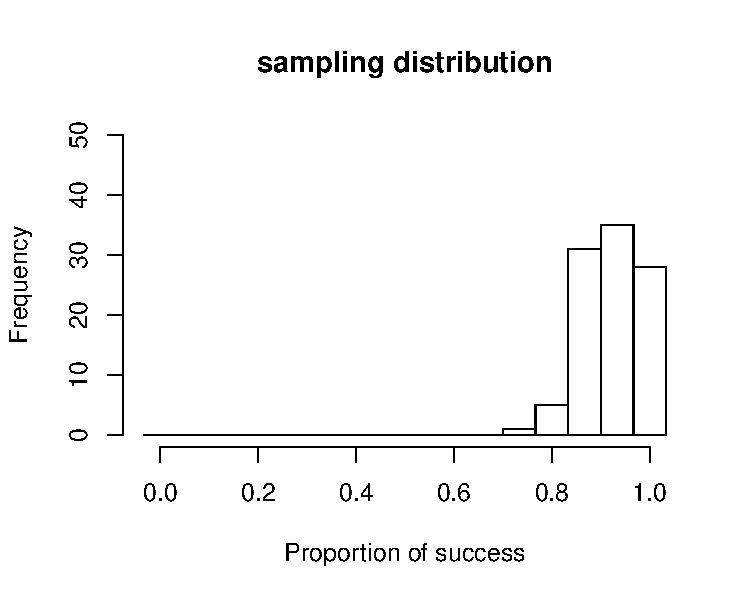
\includegraphics[scale=0.8]{code/art.pdf}
\end{center}

Of course, we might also be curious about what happens when they repeat the whole process many times. We can overlay the various histograms, using semi-transparent bars.
\begin{center}
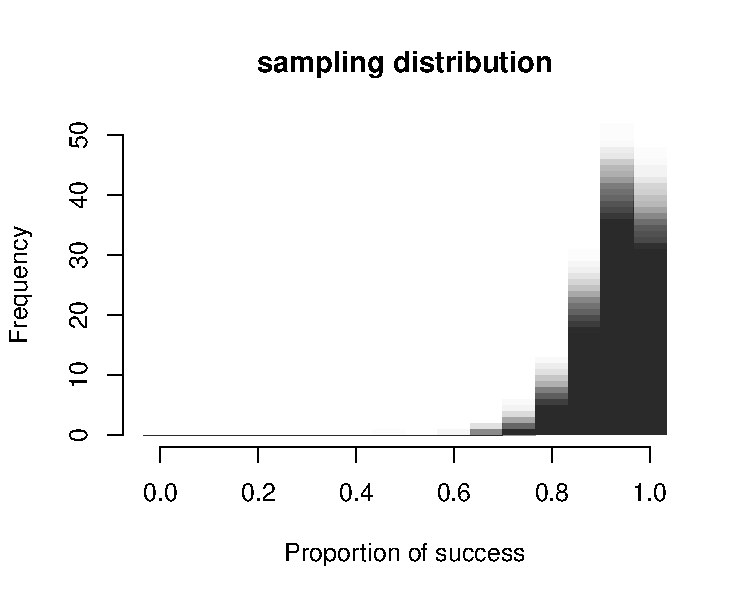
\includegraphics[scale=0.8]{code/art_many.pdf}
\end{center}
We see that we expect the distribution to be left skewed. Of course, you could have also just seen that the probability distribution of $Y$ is left skewed.

Here is my full code:
\lstinputlisting[breaklines=true]{code/art.r}
\end{enumerate}

\item In this case, the SE is going to be a scaled version of the SD of a binomial distribution. We can approach this two different ways.

First, let's find $SD(W)$. Remember, $W\sim Bernoulli(0.93)$.
\begin{center}
\begin{tabular}{|c|c|}\hline
$w_i$ & $P(W=w_i)$ \\ \hline
$0$   &  $0.07$\\
$1$   &  $0.93$ \\\hline
\end{tabular}
\end{center}
$$E(W) = \mu = (0)(0.07) + (1)(0.93) = 0.93 $$
$$SD(W) = \sqrt{(0-0.93)^2(0.07)+(1-0.93)^2(0.93)} = 0.255 $$
Also, at some point we showed that for Bernoulli variables, $\sigma = \sqrt{p(1-p)} = \sqrt{0.93\times 0.07} = 0.255$.

In general, to determine the standard error (of a sampling distribution), we divide the standard deviation of the population by the square root of $n$.

$$SE = \frac{0.255}{\sqrt{15}} = \fbox{0.066} $$

We can also remember how to calculate the standard deviation of a binomial distribution. Remember $X\sim\B{15}{0.93}$.

$$SD(X) = \sqrt{np(1-p)} = \sqrt{15(0.93)(0.07)} = 0.988$$
Now, we remember that $Y = \frac{X}{15}$. We can use a rule from Chapter 2.4.
$$Var(Y) = Var\left(\frac{X}{15}\right) = \left(\frac{1}{15}\right)^2Var(X)$$
$$SD(Y) =  \frac{1}{15}SD(X) = \frac{0.988}{15} = \fbox{0.066}$$

\end{enumerate}
\end{document}
